\begin{figure}[h]
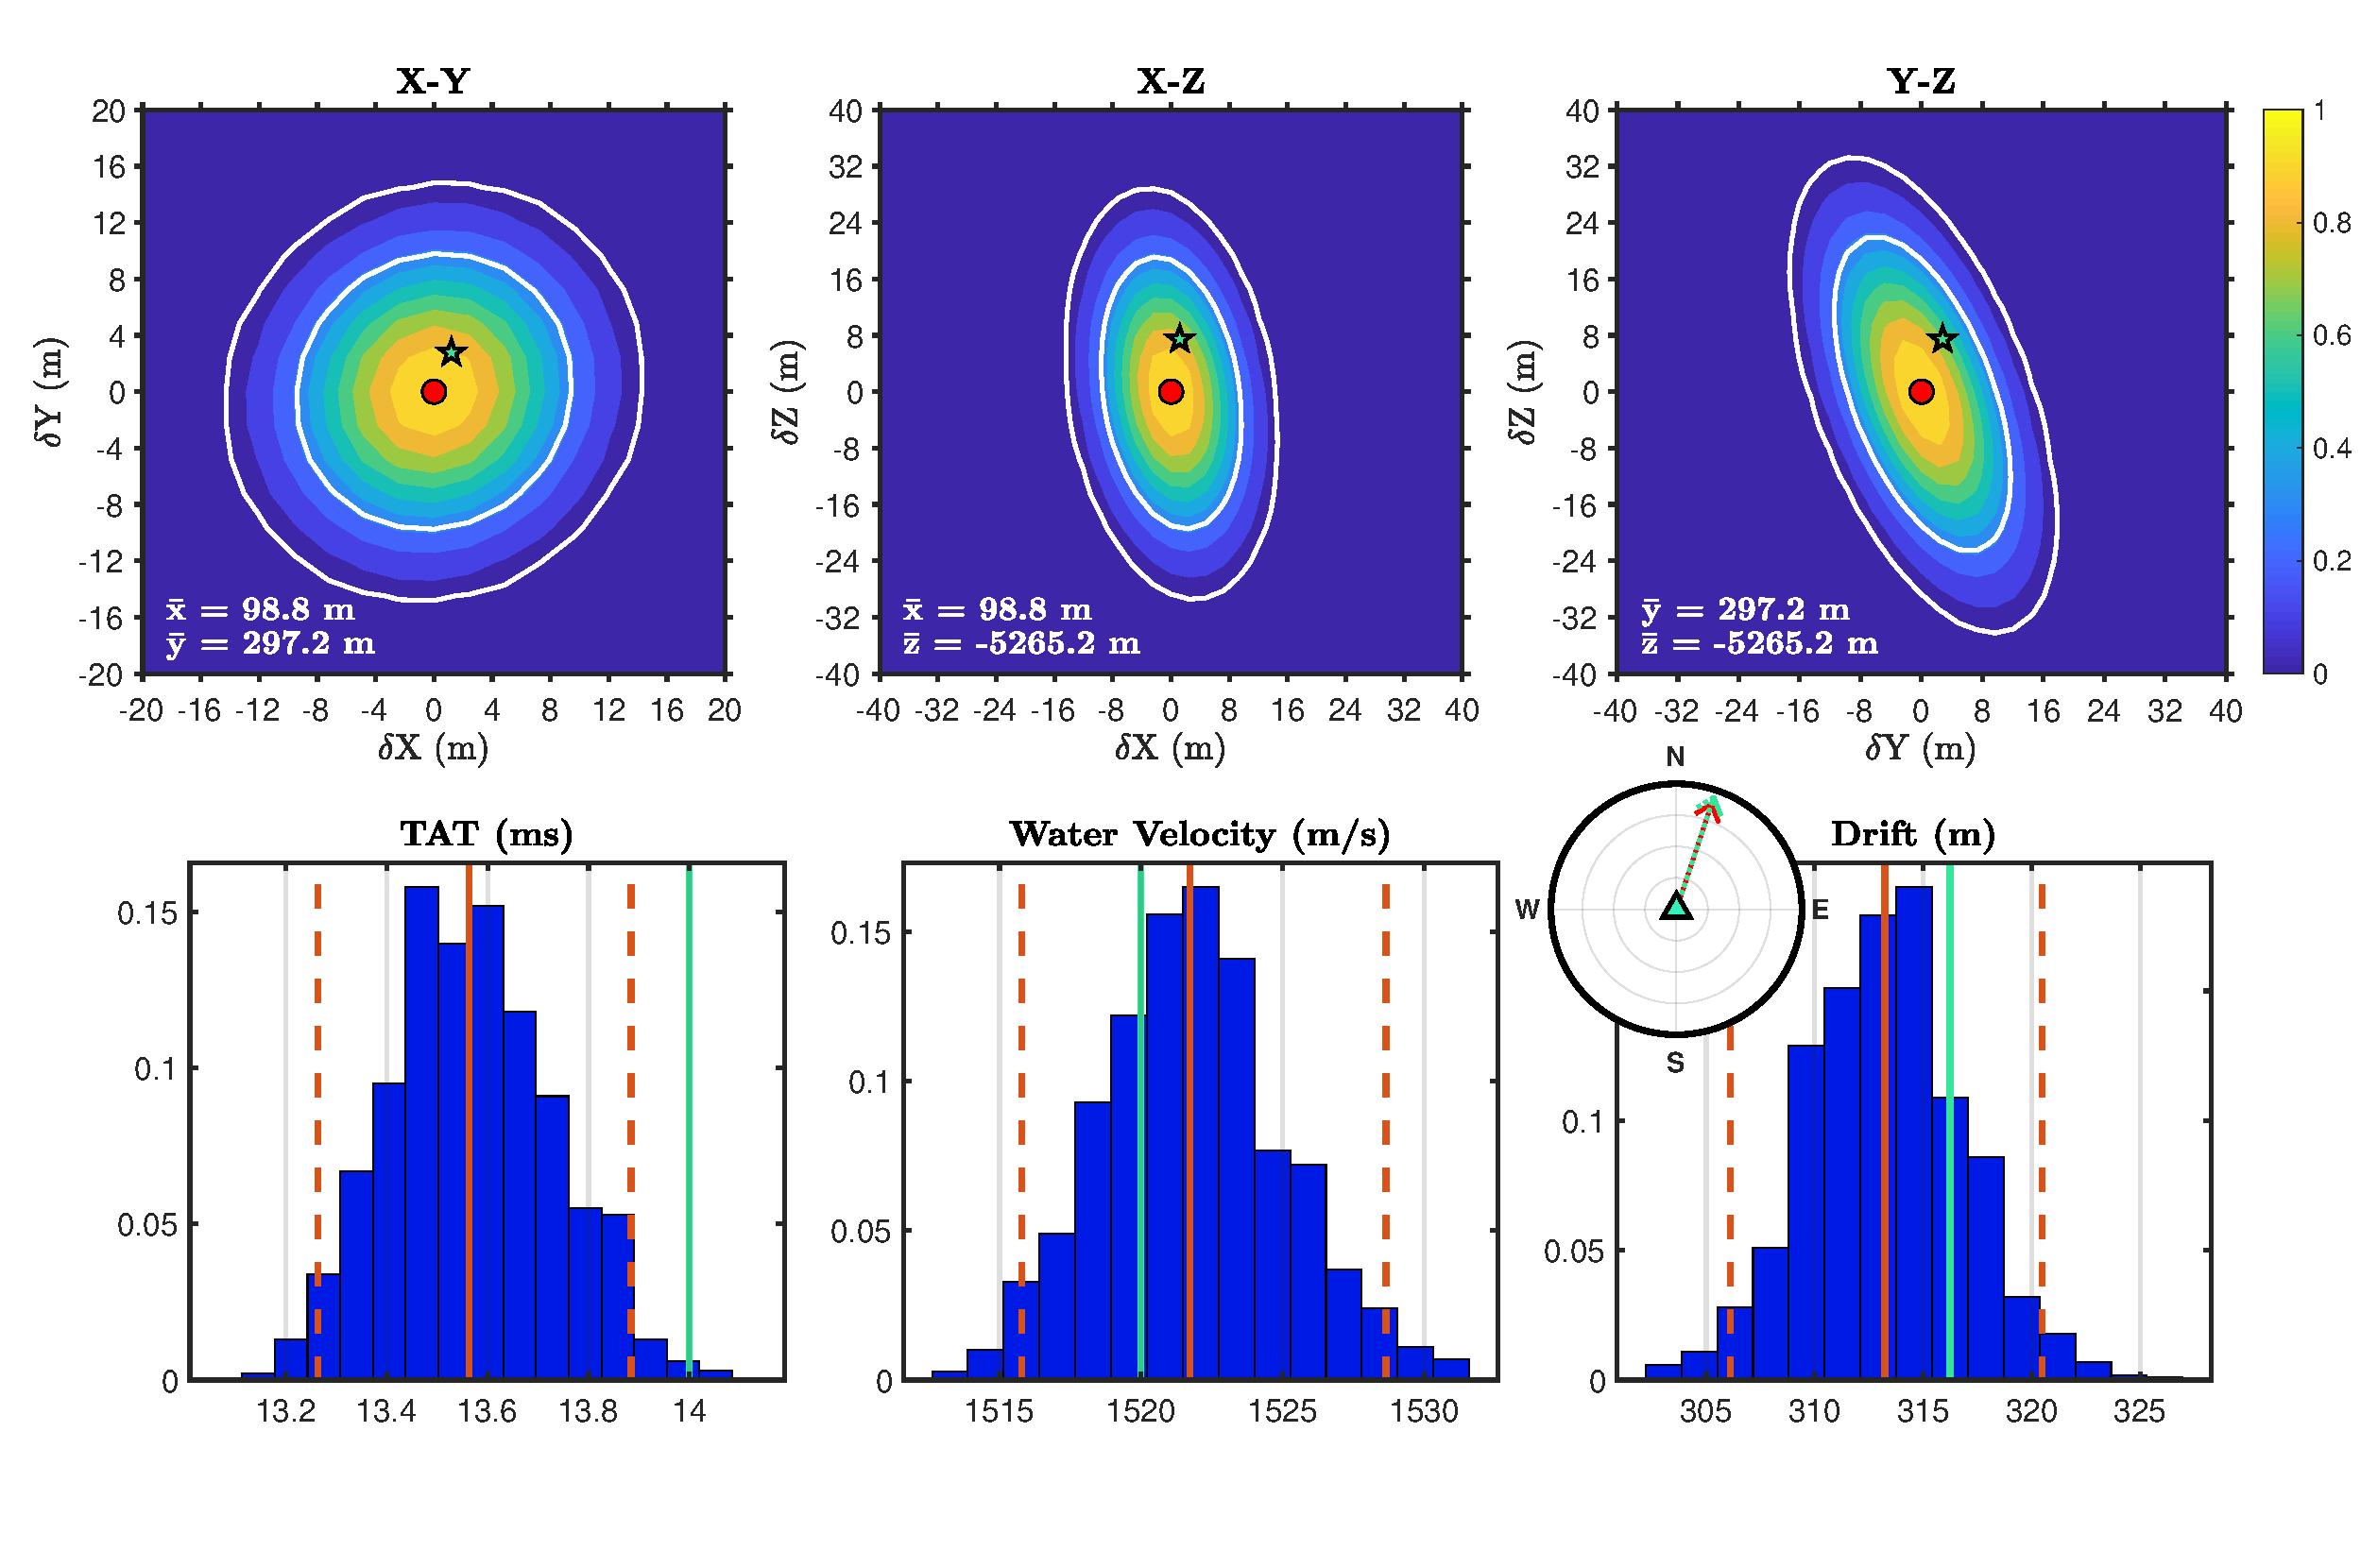
\includegraphics[trim=0cm 0cm 0cm 0cm,clip=true,width=\columnwidth]{Figure01.pdf}
\caption{Test of location algorithm using synthetic data. A comparison of the true input values (green star and lines) with the inverted model parameters (red circle and red solid lines) demonstrates that the location, depth, and water velocity are extremely well recovered, and the estimated uncertainties on these parameters are consonant with the actual misfit. Top three plots show slices through the F-test surface, contoured by probability. Bottom three plots show histograms from a bootstrap analysis with 95th percentile values indicated by dashed red lines. Inset shows the direction of true (green dashed) and estimated (red) drift with respect to the starting location. }
\label{fig:fig:one_sta_synth}
\end{figure}